\chapter{Background knowledge and related work}
\label{cha:sota}

%------------------------------------------%---------- Microservices ----------------%------------------------------------------

% TODO passar isto para o trabalho relacionado

In this chapter, we will present the concepts which serve as a basis for this thesis mainly Microservices and Virtualization. Followed by some less impactful but relevant topics such as Web Scraping and Geographical Information Systems. To end the chapter, a brief description of how successful companies are using some of these concepts and some scientific work that inspired our application.

%Upon defining the requirements and needs of the project, we began by analysing how current researchers have dealt with similar problems. For that, a search was made to find projects that contained relevant information, even if only relevant to certain sections of the problem. The following articles analyse scientific papers found that offered insights onto some of those topics:

%After understanding and breaking down the problem at hand,  analysed the current literature trying to find projects that had relevant information and could help with sections of the project.

%The first sections analyse scientific papers that offer insight into several relevant sections of the current paper, such as: microservice architecture, user interface innovation for real estate, scalability with Kubernetes.

%fter analysing the relevant literature, we will expand on to some of the relevant topics discovered through the projects, and try to compared them, if relevant, to existing technologies.

%There are multiple projects in the literature that employ a microservice architecture using kubernetes~\cite{micro_kuber}. The following paragraphs describe some of the work we found representative and relevant.

%\section{Scientific Work}
%\label{s:scientific-work}


\section{Microservices}
\label{s:microservices}
%% -- Created: 03-07-21
%% -- Last edit: 03-07-21

The microservices architecture~\cite{microservice-patterns} is based on the design of applications composed of independent processes that implement a given functionality in full, being able to function autonomously without use of another type of service, and which cooperate with each other to provide certain functionalities, while interacting through APIs.

To better understand this architecture, it is necessary to understand his predecessor, the \textbf{monolith}~\cite{monolithic-architecture}. A monolith application, as seen in Fig. \ref{fig:monolith-architecture}, is created as a single unit, split into dependent modules, which are tightly coupled to that specific application. This type of design also requires that applications have to be entirely redeployed no matter the change size. As the application grows, it becomes harder to maintain a good structure, making it harder to maintain and perform changes. 

\begin{figure}[t]
     \centering
     \begin{subfigure}[b]{0.49\textwidth}
         \centering
         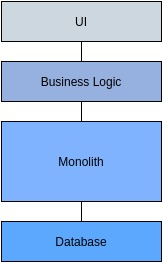
\includegraphics[width=0.5\textwidth]{Chapters/img/2_background/monolith-architecture.jpg}
         \caption{Monolith}
         \label{fig:monolith-architecture}
     \end{subfigure}
     \hfill
     \begin{subfigure}[b]{0.49\textwidth}
         \centering
         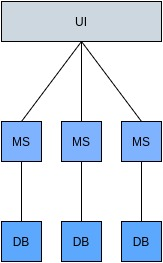
\includegraphics[width=0.5\textwidth]{Chapters/img/2_background/microservices-architecture.jpg}
         \caption{Microservice}
         \label{fig:microservice-architecture}
     \end{subfigure}
     \caption{Architectural patterns}
\end{figure}


The microservices architecture emerged from the need to overcome the limitations of the monolithic architecture, as can be seen in Fig. \ref{fig:microservice-architecture} it is composed of several services as opposed to the monolith, and each of this services has their own data stores.

\subsection{Main features}
\label{ss:microservices-features}

The microservice architecture is usually \textbf{split by business functionality}, instead of splitting them through teams such as: databases, \acrlong{ui} (\acrshort{ui}) and so on. Business functionality is usually seen as something that generates value to the company and can be independently developed, and is one of the reasons that microservices tend to be \textbf{small} and easily maintainable. They tend to be \textbf{decoupled}, which is an essential feature to easily deploy a service, without the need to coordinate with other components. To facilitate the deployment, a delivery pipeline can be put in place enabling \textbf{fast pace development with frequent small deployments}. 

As each services has a specific focus, the \textbf{technology can be tailored to the current problem}, independently of the technology used by other components. The communication between multiple components, to ensure the correct functioning, is assured through \acrlong{api} (\acrshort{api}) of neutral languague, such as \acrlong{rest} (\acrshort{rest}).

There are three main data storage patterns when it comes to data storage~\cite{9130516}: shared database, per-service pattern and Command Query Responsibility Segregation (CQRS) and Event Sourcing. In the first scenario, a single database is shared by multiple services and as such each service accesses the same global pool of data. It provides a good performance in terms of response time but does not align with the principle of loose-coupling, a fundamental aspect of the microservices design. The per-service pattern specifies that each service has a database that's dedicated only to that service. In this case, each database is in complete isolation with each service not having direct access to the data store of other services.

Finally, CQRS represents a way to split data access into two distinct parts the commands which represent operations that modify the state of the data and queries which represent read-only requests for data.

%Unlike monolithic architectures, where a single database is shared by everyone, in the microservices architecture, each business functionality with a corresponding service, has \textbf{their own database}.  

\subsection{Advantages}
\label{ss:microservices-advantages}

% Technology heterogeneity, resilience, scalability,  fast deployment, faster onboarding, easy refactoring

As stated previously, \textbf{technology heterogeneity} is one of the main advantages of the microservices architecture~~\cite{technology-heterogeneity}. It opens up the door to the use of multiple technologies, old or new, in each component always focusing in improving the performance. It extends to data stores as well, since each service has it's own database, it can use the most suited solution such as non-relational databases or a  graph-oriented database. This architecture, in conjunction with component decoupling, also allows for a faster adoption of this technologies, since it affects only a small part of the system.

The fact that the systems are decoupled and independent, allows them to endure failure. If one component fails, the system can continue operation with the exception of that specific component, making this architecture \textbf{resilient}. Easier access to a \textbf{scalable} solution is also one of its main advantages, by having smaller services, if any of them ever become overloaded, it is easier to scale. 

Since services have \textbf{fine granularity}, and by nature smaller \gls{codebase}s, it makes substitution and rewriting of components easy, by reducing the associated risk and cost. A smaller \gls{codebase} also helps with the onboarding process of new hire and an improved workload distribution. By assigning smaller codebases to teams, it allows them to have a \textbf{more focused task force}.

During production it may happen that services become overloaded, which can easily be dealt by \textbf{scaling} the affected services. This type of management saves money compared to a monolithic architecture, since in the latter, it would be necessary to scale the entire system. As \textbf{services are independently deployed}, changes happen faster and the risk associated with those changes is lower. But, even in worst case scenarios, the origin of the problem can be found fast and a rollback performed to previously working versions. For the same reasons, it also becomes \textbf{easy to add new features}~\cite{9213058}.

\subsection{Challenges}
\label{ss:microservices-challenges}

With so many moving pieces the microservices architecture introduces many factors that must be taken in consideration, such as:

\paragraph{\textbf{Design}} When creating microservices for the first time, it might be hard to determine: microservice's size, connection points between each service and how to integrate all of them. As such, designing this services assumes a deeper knowledge of the domain, where each microservice should encapsulate, clarify and clearly define specific requirements~\cite{microservices-challenges-1}.

\paragraph{\textbf{Security}} Microservices are usually deployed across multi-cloud environments, resulting in increased risk and loss of control of application components. Data security~\cite{data-security} within microservices is also a concern, as data flows between multiple components and, possibly, public clouds, it becomes difficult to maintain confidentiality, integrity, and privacy of user data~\cite{microservices-challenges-2}.

\paragraph{\textbf{Testing}} Given the granularity of components and their need to communicate with each other, it becomes increasingly difficult to keep up with all of the services interactions when performing integration tests.

\paragraph{\textbf{Monitoring}} %Given the nature of deploying microservices in independent containers or \acrshort{vm}, it can become difficult to measure performance of multiple interactions from the user request to the end of the transaction. As such, a good monitoring solution must be configured in conjunction with good logging practices.

Due to the nature of microservices, when put together within a containerized environment they become a system with many moving parts resulting in massive amounts of data from multiple sources.

In addition to it, with the increasing number of new libraries, tools and new frameworks to build software systems, such as web servers, databases, queues and so on. It turned the system architecture into a composite of multiple third-party pieces. As such, systems now need to provide integration with a large and dynamic ecosystem to provide complete observability.

This level of observability is only possible with a precise, fine-grained, and safe monitoring system. The goal of such a system is to monitor/manage, through the analysis of metrics of the various activities in the cloud, obtained with good logging practices.

\paragraph{\textbf{Communication}} microservices act as a small standalone application that sometimes have to communicate with each other. There's two main approaches to solve this problem:

\begin{enumerate}
    \item \textbf{Asking the service directly:} for this approach, the client interacts directly with the microservices through an exposed endpoint usually going through a \gls{load-balancer}. The requests are then distributed between the multiple instances of that service. This approach has the disadvantage of requiring users to perform multiple requests to different microservices to obtain the required data, thus introducing latency to the operation. 
    \item \textbf{Using an API Gateway:} it is a server that handles all the clients requests, it abstracts the internal architecture from the user being the only way to interact with the system, serving as an extra layer of protection. It is also possible to aggregate results if a request requires data from multiple services, which allows to reduce the load that the customer places on the system and also, simplifies the code at the client. As a drawback, it introduces a bottleneck capacity and developer wise. For capacity, it makes every single request go through it with the possibility of overloading it and development wise, it requires a common deployment point between every microservice. But overall, it ends being the best option for direction communication.
\end{enumerate}

\acrlong{ipc} (\acrshort{ipc}) is used when microservices must communicate with each other. There are a variety of client -- service interaction styles that can be categorized along two dimensions:

\begin{enumerate}
    \item \textbf{Number of services involved:} if a client request is processed by exactly on service instance (one-to-one) or if each request is processed by multiple service instances (one-to-many);
    \item \textbf{Synchronous or asynchronous interaction:} if the client expects a timely response, and mighty even consider blocking while it waits, it is a synchronous interaction. And asynchronous if the client doesn't block while waiting for a response, and the response, if any, isn't necessarily sent immediately.
\end{enumerate}

These dimensions can then be combined to form the multiple interaction styles presented in Table \ref{tab:nginx-microservices}.


%\begin{table}[H]
%    \centering
%    \begin{tabular}{|c|c|c|} 
%    \cline{2-3}
%    \multicolumn{1}{c|}{}         & \textbf{one-to-one}& \textbf{one-to-many} %    \\ 
%    \hline
%    \textbf{synchronous}                   & Request/Response   & -            %     \\ 
%    \hline
%    \multirow{2}{*}{\textbf{asynchronous}} & Notification       & Publish/subscribe   \\ 
%    \cline{2-3}
%                                  & Req/async response & Publish/async responses  \\
%    \hline
%    \end{tabular}
%    \caption{\acrshort{ipc} styles~\cite{nginx-microservices}}
%    \label{tab:nginx-microservices}
%\end{table}

\begin{table}[t]
\caption[Inter-process communication styles]{\acrshort{ipc} styles~\cite{nginx-microservices}}
    \label{tab:nginx-microservices}
    \centering
    \begin{tabular}{c c c} 
    \toprule
    \multicolumn{1}{c}{}         & \textbf{one-to-one}& \textbf{one-to-many}     \\ 
    \cline{2-3}
    \textbf{synchronous}                   & Request/Response   & -                 \\ 
    \hline
    \multirow{2}{*}{\textbf{asynchronous}} & Notification       & Publish/subscribe   \\ 
    \cline{2-3}
                                  & Req/async response & Publish/async responses  \\
    \bottomrule
    \end{tabular}
    
\end{table}
\begin{enumerate}
    \item \textbf{Request/Response:} the client makes a request and waits for a response, might block while waiting;
    \item \textbf{Request/async response:} the client makes a request and the service replies asynchronously. The client is design with the assumption that the response might take a while, and as such does not block while waiting;
    \item \textbf{Publish/Subscribe:} the client publishes a message and it is consumed by previously subscribed services;
    \item \textbf{Publish/Subscribe async:} the client publishes a message and waits for a response from the subscribed services;
    \item \textbf{Notification:} a client sends a request to service but expects no reply;
\end{enumerate}

As message-driven communication is done asynchronously, the messages need to wait somewhere to be processed. \textbf{Message brokers} fulfill this role, by helping the system guarantee that messages will be processed, even if in a slower way. It allows applications and services to communicate with each other and exchange information by converting messages between formal messaging protocols, which allows independent services to ``talk'' to each other directly, even if they were written in different languages or platforms.




%\section{Communication models}
%\label{ss:message-brokers}

% What is a message broker
%\todo[inline]{what is a broker, desenvolver mais}
%Message brokers is a software that enables applications, systems, and services to communicate with each other and exchange information by converting messages between formal messaging protocols. This allows interdependent services to "talk" to each other directly, even if they were written in different languages or platforms.
%\subsection{Request/Response}
%\subsection{Publish/Subscribe}
%\subsubsection{AMQP}
%\subsubsection{MQTT}




%------------------------------------------%------------ Virtualization ---------------%------------------------------------------

\section{Virtualization}
\label{s:virtualization}
%% -- Created: 03-07-21
%% -- Last edit: 03-07-21

"Virtualization, is the abstraction of computer resources"~\cite{virtualization-basics}. It is a technology which allows the creation of multiple simulated environments from a single physical hardware system. 

The possibility of having the virtual instance of a server in a layer abstracted by hardware from the host, solves the problem of inefficiency of using one server per application. From the perspective of the application which is ran in the \acrshort{vm}, the environment is the same as a physical server where the \acrlong{so} (\acrshort{so}), libraries and applications are unique and independent from the hosts \acrshort{so}. 

Virtualization is split into four key properties~\cite{virtualization-key-properties}, with the corresponding benefits:

\begin{itemize}
    \item \textbf{Partitioning:} Run multiple operating systems in one physical machine and divide system resources between \acrlong{vm}s;
    \item \textbf{Isolation:} Provide fault and security isolation at the hardware level while also preserving performance with advanced resource controls;
    \item \textbf{Encapsulation:} Save the entire state of a virtual machine to files and be able to move and copy virtual machines as easily as moving and copying files;
    \item \textbf{Hardware Independence:} Provision or migrate any virtual machine to any physical server.
\end{itemize}

Hypervisor~\cite{hypervisor} is the software responsible for creating and managing \acrshort{vm}s. It allows one host computer to support multiple guest \acrshort{vm}s by virtually sharing its resources, such as memory and processing. There are two main hypervisor types:

\begin{itemize}
    \item \textbf{Type 1} ("bare metal"): acts like a lightweight operation system and runs directly on the host's hardware;
    \item \textbf{Type 2} ("hosted"): runs as a software layer on an operation system, like other computer programs.
\end{itemize}

Even though \acrshort{vm}s solve a number of problems they are not perfect, as each \acrshort{vm} requires a dedicated \acrshort{so} which consumes \acrlong{cpu} (\acrshort{cpu}), \acrlong{ram} (\acrshort{ram}) and disk space, which could have a better use. %Additionally, boot up speed, portability and licence requirements drove users to the creation of alternatives, such as \textbf{containers}.

%------------------------------------------%------------ Containers -----------------------------------
%\subsection{Containers}
%\label{ss:containers}
%% -- Created: 03-07-21
%% -- Last edit: 03-07-21

\paragraph{Containers} alternatively, provide isolation and resource management, with the term being derived from shipping containers -- a standard method to store and ship supplies. A container consists of an entire runtime environment which packages an application's components as building blocks of the complete application, with includes: dependencies, libraries, binaries and configuration files all bundled into one package. This allows the container to become isolated from the \acrshort{so} from the machine who hosts the container~\cite{virtualization}. 

\begin{figure}[t]
    \centering
    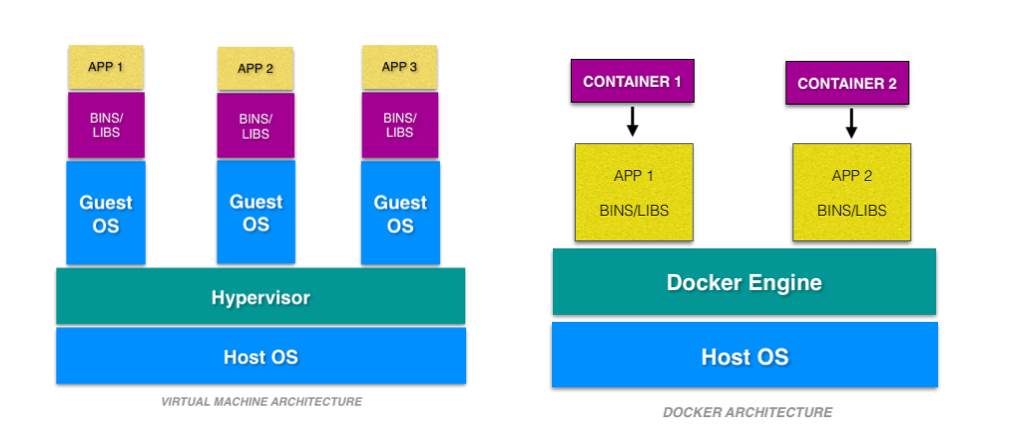
\includegraphics[width=1\textwidth]{Chapters/img/2_background/docker-vs-vm.png}
    \caption[Virtual machine and container comparison]{Virtual machine and docker container comparison ~\cite{docker-vs-vm-table}}
    \label{fig:docker-vs-vm}
\end{figure}

Containers are much more lightweight, allowing for a higher number of software components when compared with \acrshort{vm} who need to run its own set of system processes, requiring additional resources. A container, on the other hand, is nothing more than a single isolated process running in the host OS, consume only the required resources.

Since they don't require their own \acrshort{so}, as shown in Fig.~\ref{fig:docker-vs-vm}, it has a smaller burden in the system by saving resources such as \acrshort{cpu}, \acrshort{ram} and storage. Given the fact that all dependencies are packaged, it allows for a possible abstraction between the application and the environment where it is executed, resulting in a decoupling between the application and the system \acrshort{so}, allowing for higher portability and consistency. A more in-depth comparison can be seen in Table \ref{tab:docker-vs-vm}.

\begin{table}[t]
     \caption[Virtual machine and container comparison]{Virtual machine and container comparison ~\cite{docker-vs-vm-table} } 
    \label{tab:docker-vs-vm}
    \centering
    
    \begin{tabular}{p{0.2\textwidth} p{0.35\textwidth} p{0.35\textwidth}}
       \toprule
        Parameter     & Virtual Machines  & Containers                                                                                \\ 
        %\hline
        %\hline
        \midrule
        Guest OS      & Each VM runs on virtual hardware and Kernel is loaded into in its
        own memory region                            & All the guests share same
        OS and Kernel. Kernel image is loaded into the physical memory  \\ \addlinespace 
        %\hline
        Communication & Via Ethernet Devices  & Standard IPC mechanisms like Signals, pipes, sockets etc.     \\ \addlinespace
        %\hline
        Security      & Depends on the implementation of Hypervisor   & Mandatory access control can be used   \\ \addlinespace
        %\hline
        Performance   & Emulation of hardware, resulting in a bigger overhead & Containers provide near native performance as compared to the underlying Host OS.         \\ \addlinespace
        %\hline
        Isolation     & Sharing libraries, files etc between guests and between guests hosts not possible.   & Linux Namespaces and Control Groups, make sure each process sees its own personal view of the system and limit resource consumption   \\ \addlinespace
        %\hline
        Startup time  & VMs take a few mins to boot up  & Containers can be booted up in a few secs as compared to VMs     \\ \addlinespace
        %\hline
        Storage       & VMs take much more storage as the whole OS kernel and its associated programs have to be installed and run     & Containers take lower amount of storage as the base OS is shared  \\                \bottomrule       
    \end{tabular}

   
\end{table}

%------------------------------------------%-------------Virtual Machines -----------------------------

%------------------------------------------%------------ Orchestration ---------------%------------------------------------------
\subsection{Container orchestration}
\label{ss:container-orchestration}
%% -- Created: 14-10-20
%% -- Last edit: 04-07-21

Container orchestration automates the deployment, management, scaling and networking of containers. It helps with the deployment of the same application across different environments without the need of redesigning it. Although they introduced new problems to the applications running in these containers, as it becomes necessary to figure our how to monitor an application, how to update it without disrupting the service, scaling, handle errors while running and even how to restart it~\cite{kubernetes-vs-docker}. All of this led to the emergence of \acrfull{coe}s.

These engines are able to perform fundamental operations with containers, such as ensuring coordination, controlling and monitoring, while also being able to manage the applications themselves. They are responsible for abstracting resources from the applications, so system resources are abstracted from the containers than run on them~\cite{containerization-overview}.

Docker Swarm and Kubernetes are the most popular, and share the following high-level features~\cite{Casalicchio2019}:

\begin{itemize}
    \item \textbf{Container scheduling:} responsible for starting and stopping containers, distributing resources between them, recover from failure, scaling applications (manually or automatically) and rebalancing containers from failed hosts to healthy ones;
    \item \textbf{High Availability:} assuring the availability of the application, containers or even the orchestration system itself;
    \item \textbf{Health checks:} determine container or application health;
    \item \textbf{Service discovery:} determining where services are located on the network in a distributed architecture;
    \item \textbf{Load Balancing:} distribute requests, either internally generated in a cluster or from external clients. 
\end{itemize}

It is important to clarify that even though they are related, there's a difference between automation and orchestration. Automation streamlines the process by reducing human interaction with the system and introducing software that allows a reduction in cost, complexity, and error. In general, automation is usually associated with performing one single task. This is different from orchestration, which is how you can automate a process that involves several steps across multiple systems. With the processes now automated, it is possible to orchestrate them to run automatically.




%------------------------------------------%------------ Monitoring ---------------%------------------------------------------
%\section{Monitoring}
%\label{s:monitoring}
%% -- Created: 03-07-21
%% -- Last edit: 05-07-21



%The following sections look into some possible tools to monitor these systems.

%------------------------------------------%------------ Prometheus -----------------------------



%Redis is an in-memory operating key-value store for strings, hashes, lists and sets \cite{Sanfilippo:2016}. The 2009 released open-source database allows range queries and has built in Lua support for scripting. Due to its low data structure complexity, Redis provides large performance advantages in comparison to relational databases. Snapshotting or append only files allow on-disk persistence of the in-memory stored data. Later versions also allow distributed storage across clusters. Redis provides driver bindings for the most prevalent programming languages.

%Redis [19], is an open source, in-memory data structure store, used as non-relational database, cache, and message broker, developed by Salvatore Sanfilippo in 2009. It supports replication to scale read performance, in-memory persistence storage on disk, and client-side sharding [56] to scale write performance. Redis stores a mapping of keys to five different types of values: strings, list, sets, hashes, and sorted sets. It supports writing of its data to disk automatically in two different ways: dumping the dataset to disk every once in a while (Snapshotting), which is not very reliable due to possible system shutdowns or power fails, or by appending each command to a log (Append-only file), which is a fully-durable and reliable strategy. Also, it supports publish/subscribe, master/slave replication, and scripting (stored procedures). Redis is written in C and works in most POSIX systems, such as Linux, *BSD and OSX. It can be used through APIs for most programming languages, such as Java, C, C++, C, PHP, among others.


%Redis is a data structures server, while in traditional key-value stores you associate string keys to string values, in Redis the value is not limited to a simple string, but can also hold more complex data structures.

%The keys are binary safe, which means that any binary sequence can be used from a simple three character string to the content of a JPEG file. \\

%For values, Lists were the relevant data structure for this project. The term List is often used in an improper way, for instance, python lists are not what the name may suggest (Linked Lists), but rather Arrays. From a general point of view a List is just a sequence of ordered elements, but the properties of a list implement using an Array are very different from the properties of a List implement using a Linked List.

%Redis lists are implement via Linked Lists, this means that even if the current list has millions of elements, the operation of adding a new element in the head or tail is performed in constant time, so the time it takes to add an element to a list of ten elements is the same as a list with ten million.

%Of course there's a downside, accessing elements by index is very fast (constant time indexed accesses) with lists implemented with an Array and not so fast in lists implemented by linked lists (where the operation required an amount of work proportional to the index of the accessed element).

%Since the main purpose of Redis in this project is to be used as Queue, with a consumer-producer pattern where the producer pushes items into a list, and a consumer consumes those items to execute their actions, this type of data structure ends up being an advantage.


%--------------------------%--------------Web scraping----------------------------%------------------------------------------
\section{Web scraping}
\label{s:web_scraping}

Web scraping refers to the extraction of data from a website, this information is collected and then, possibly exported, into a more useful format for the user. This became a necessity as the quantity of data shared and consumed is constantly growing. From the principle techniques available for data extraction, this work will focus on the technique of data extraction through \acrlong{xml} \textit{path language} (\acrshort{xpath}).

Xpath is a technique which requires the user to analyse in detail either the HTML tree or \acrlong{dom} (\acrshort{dom}) of the page he intends to scrape. After this analysis, the user picks the data he wishes to extract and draws a path to it, with the help of the XPath language. This type of technique is extremely sensible to changes, for this reason the user needs to constantly check for modifications on the source. \\

Since web scraping may cause pages to overload with many requests and other possible issues, an \textit{internet etiquette} must be maintained~\cite{6623484}, following rules such as request limitation and behaving like a normal user. To deal with scrapers, most websites define this rules in their \textbf{robot.txt} file, which can be usually found by appending the filename to the URL (e.g., imovirtual.com/robots.txt). In this file, the owners of the domain may define which endpoints may be scraped, what type of User-agents are allowed, access to files, etc... Along with this file, the website's Terms \& Conditions page will usually have information regarding their data scraping policy.

In the next subsections, some of the tools used to apply this techniques will be presented.


%scraping vs crawling relevante comparar?
%importancia de data collection?


%------------------------------------------%---------- Databases ----------------%------------------------------------------

\begin{comment}

\section{Databases}
\label{s:databases}

This chapter introduces important database concepts, while also going over
different ways of thinking about data storage, while also understand different storage models for concepts such as \acrfull{nosql}.


%----------------%------------ CAP THEOREM -----------------------------
\subsection{CAP theorem}
\label{ss:cap-theorem}

The CAP theorem was initially a conjecture made by computer scientist Eric Brewer. It's fairly useful way to think about tradeoffs in the guarantees that a system design makes. The theorem states that of these three properties:

\begin{itemize}
\item \textbf{Consistency}: all nodes see the same data at the same time;
\item \textbf{Availability}: node failures do not prevent survivors from continuing to operate;
\item \textbf{Partition Tolerance}: the system continues to operate despite message loss due to network and/or node failure.
\end{itemize}

only two can be satisfied simultaneously, as illustrated on Figure \ref{fig:cap-theorem}.

%https://www.researchgate.net/figure/Visualization-of-CAP-theorem_fig2_282679529
\begin{figure}[h]
	\centering
	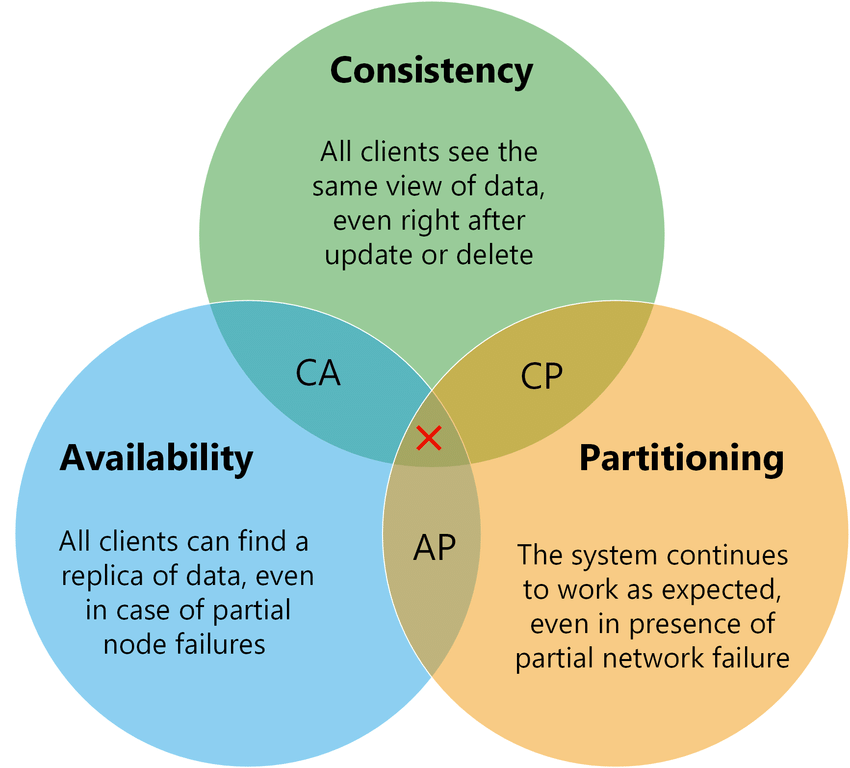
\includegraphics[width=0.5\linewidth]{Chapters/img/2_background/CAP-theorem.png}
	\caption{CAP theorem~\cite{cap-theorem-figure}}
	\label{fig:cap-theorem}
\end{figure}

Based on this, three different system types emerge: Consistency \& Availability (CA), Consistency \& Partition Tolerance (CP) and Availability \& Partition Tolerance (AP). 

The CA and CP system designs both offer the same strong consistency. The only difference being that a CA system cannot tolerate any node failures, while a CP system can tolerate up to \textit{f} faults as long as the majority f+1 stays up. This happens because the CA system stops accepting writes as soon as a node or network failure is detected, since it can identify the type of failure it stops accepting writes. 

While the CP system prevents divergence (e.g. maintains single-copy consistency) by forcing asymmetric behavior on the two sides of the partition. It only keeps the majority partition around, and requires the minority to become unavailable (e.g. stop accepting writes), which retains a degree of availability and ensures single-copy consistency.

With AP, the distributed system are always available and tolerate partitions maintain their service even when partitions occur. However, a reachable node may then hold (temporarily) inconsistent state. Thus, this intersection of properties is also known as eventual consistency. In terms of data and state, the sacrifice of strong consistency guarantees appears to be questionable at first glance. However, many applications can indeed tolerate deferred consistency properties when favoring availability at all costs. In this case, it is important to keep in mind potential issues due to eventually consistent data on application level during development.

\subsection{Relational}

Relational databases or \acrfull{rdbm} are storage systems based on the relational model first specified by E. F. Codd~\cite{Codd1970ARM}. Nowadays this type of databases follow the SQL standard, which imposes formal rules on how the data should be manipulated and queried.

\begin{figure}[h]
    \centering
    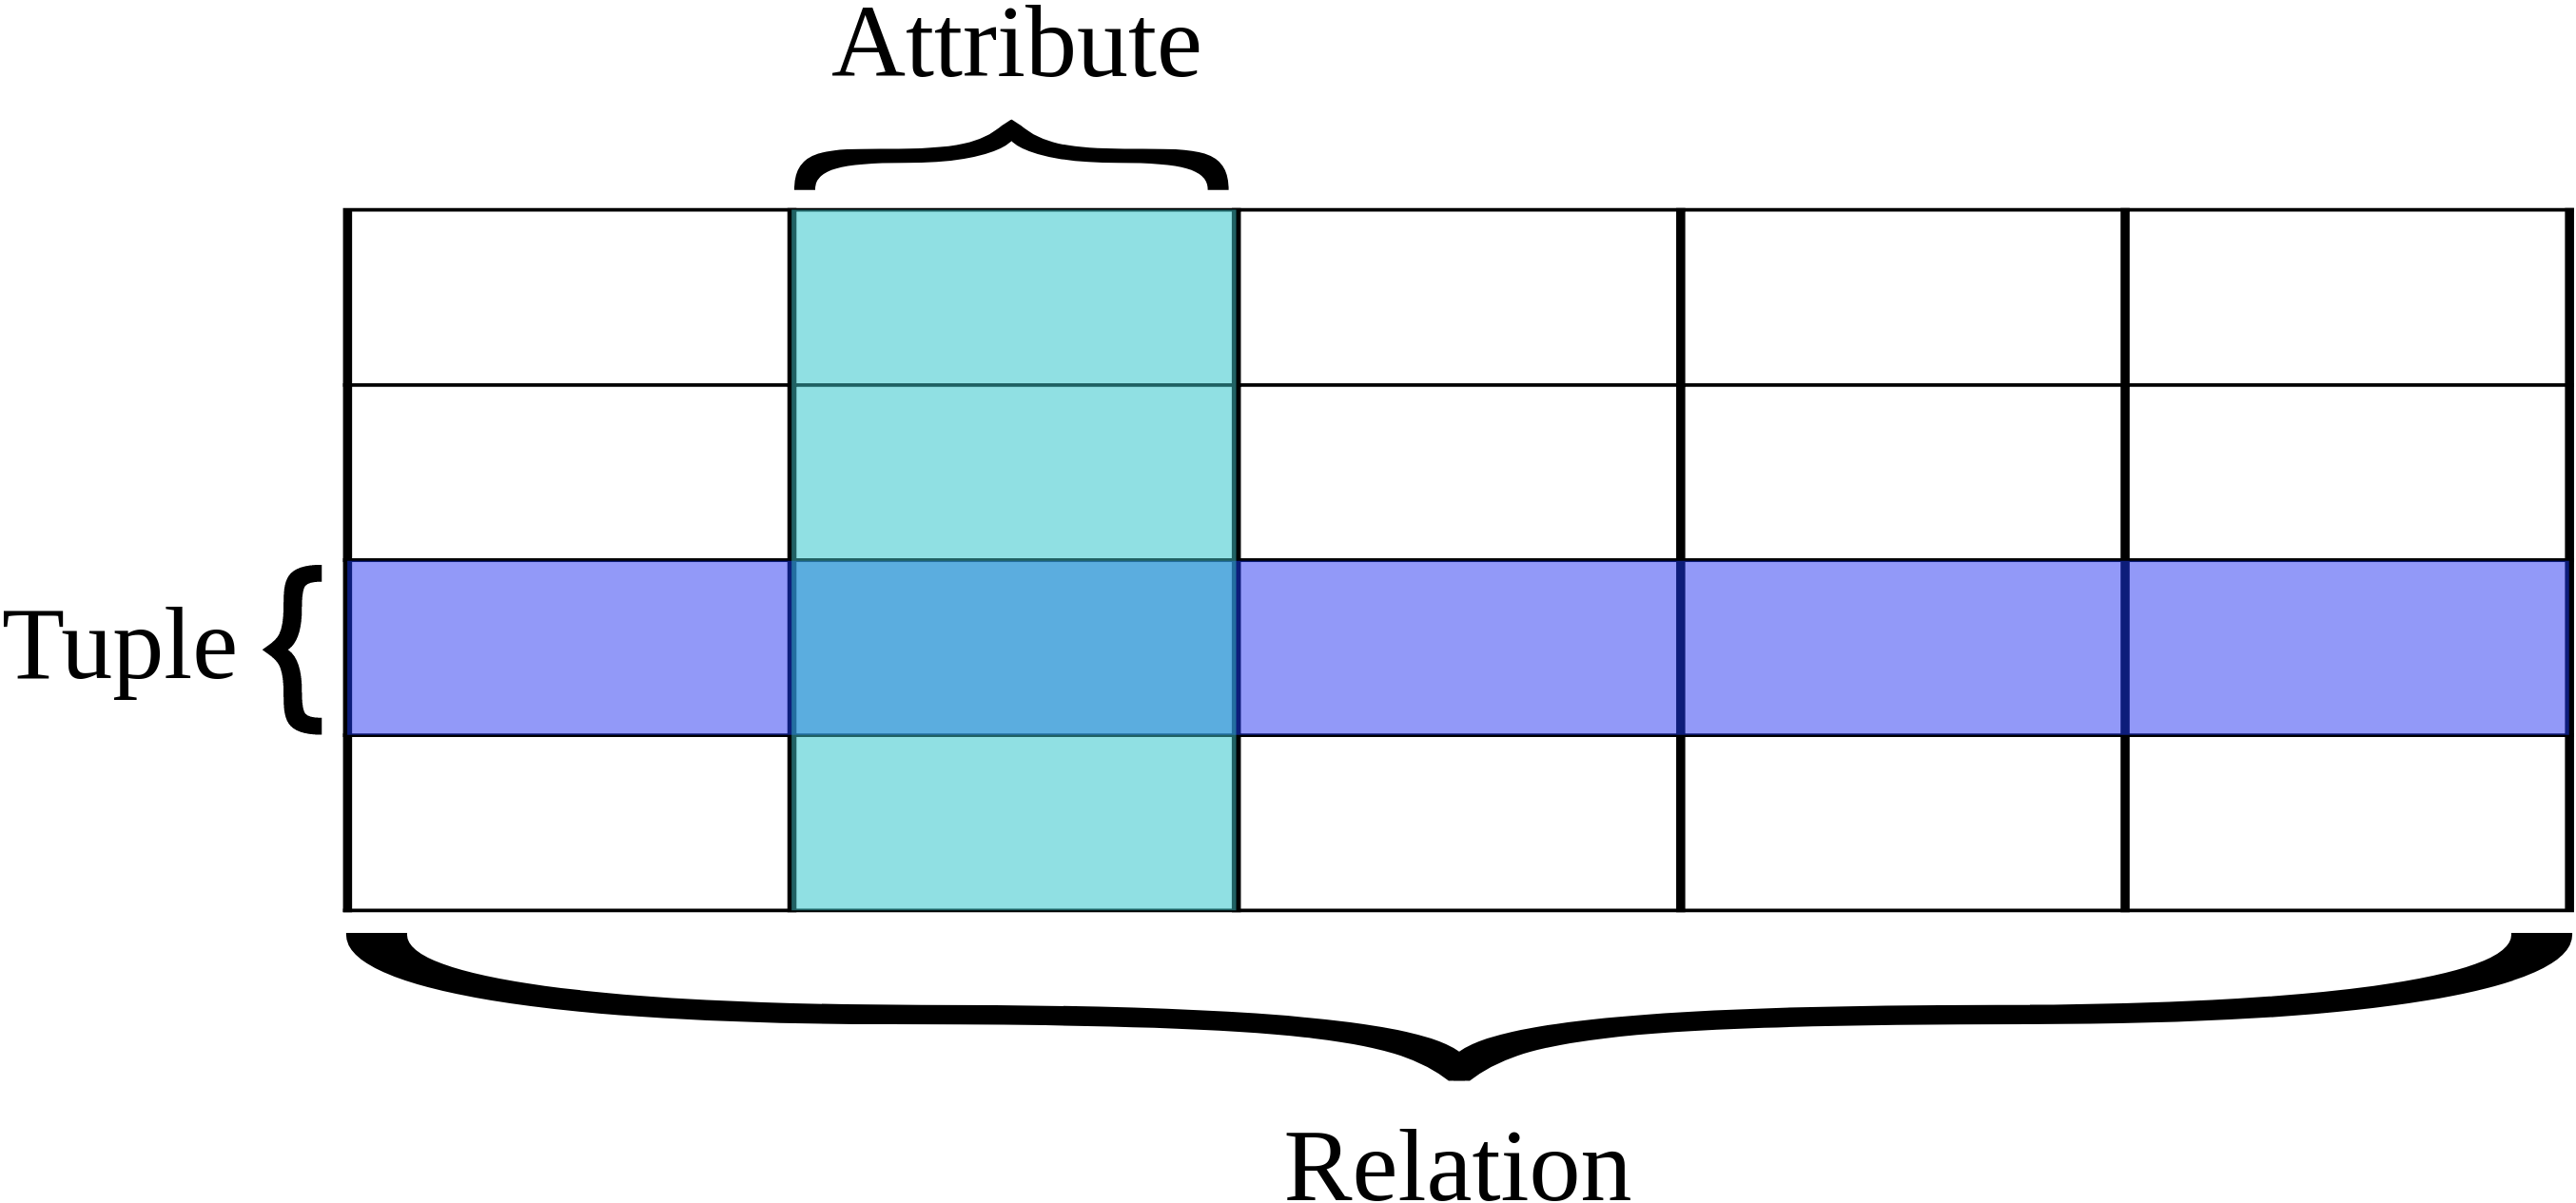
\includegraphics[width=0.75\textwidth]{Chapters/img/2_background/relational-table-example.png}
    \caption{Relational model table} 
    \label{fig:relational-model-table}
\end{figure}


In the \textbf{relational data model}, all data entries are represented in tuples which are then grouped into relations. More accurately, data is organized into tables called relations representing an entity, and each of its records are called a tuple. Table columns are usually called attributes and form the basis for the types of queries that can be performed over tables, an example of this can be seen in Fig. \ref{fig:relational-model-table}.

Each relation has a subset of attributes known as \textbf{candidate keys} that uniquely identify each tuple in the relation, the minimal subset of this attributes is called a primary key. As a way to create connections between tables, a table may \textbf{foreign keys}, which are primary keys from different tables.

Data is normally indexed by their primary key as it is the most efficient way of data retrieval, but sometimes it is necessary to access data from other attributes in those cases, this attributes can also be indexed.

This type of databases usually provide transactional support with different levels of isolation, which is particularly useful for application programmers, as it becomes easier to understand and maintain a coherent application state. Transactions are conceptually arbitrarily complex operations over data that feature what is commonly denominated as ACID properties, which is an acronym for the following properties:

\begin{itemize}
    \item \textbf{Atomicity}: it must be ensured that every transaction is not partially executed under any circumstances (i.e., system crashes or power failure). If a transaction contains an instruction that fails, then the whole transaction must fail and the database must be left unchanged.
    \item \textbf{Consistency}: any change must not break the database. This means that a successful transactions makes the database transition between two correct states, and any data written must follow all the applicable rules including referential integrity, triggers, etc.
    \item \textbf{Isolation}: the transactions should be isolated and not interfere with each other, as such, two concurrent transactions cannot modify the same data.
    \item \textbf{Durability}: the system must ensure that once transactions are committed, they are stored in a fault tolerant way, and their effects will not be forgotten.
\end{itemize}


\subsection{NoSQL}
\label{ss:nosql}

Relational databases are seen as a traditional choice given their popularity over the years, but a big obstacle arose thanks to the large amount of data being produced and its uniformity. Although \acrshort{rdbm}s are capable of managing all types of data: structured, semi-structured, and unstructured; managing it poses new challenges. Semi-structured data requires data to be processed and converted in relational data, while unstructured data has to be saved as a blob object and not stored directly. This non-uniformity of data led to the creation of \acrshort{nosql}, databases that are highly scalable and efficient, while providing great horizontal scalability~\cite{8284494}.

Any storage system that does not follow the SQL standard can be considered a NoSQL database, as such it is difficult to categorize these systems. The following sections present an overview of generally agreed upon categories.


\subsubsection{Key-value}
\label{sss:key-value-store}

This category uses a storage structure similar to HashMaps, key-value stores prioritize low read-write latency and availability over consistency, made possible by using a simple but efficient data structure that accesses data in constant time.

The key is a uniquely indexed identifier that is assigned to the value of the record, the value itself can be stored in multiple formats such as sets, lists, arrays, bitmaps and \acrshort{json} which facilitates the storage of unstructured and semi-structured data. The simplicity of the data structure also brings some disadvantages, as this model is not optimized to lookup values, requiring either scanning the whole collection for the desired attribute or creating separate index values.

Key-value stores favor persistency in data storage and are ideal for e-commerce applications that require quicker retrieval of data, stock trading aswell as the data is usually associated with a stock ticker.

\subsubsection{Document}
\label{sss:document-store}

This type of system store data in the form of semi-structured sets of key-value pairs, known as documents, encoded into standard formats such as \acrshort{xml}, \acrfull{json} and \acrfull{bson}. A document is treated as a unit similar to an object or a record, except that it is self-describing, meaning that a set of (name, value) pairs are stored together in a document.

Each document is processed without breaking down into atomic key-value pairs, allowing for complex querying such as aggregation. Data is indexed through the document id, which works as a primary identifier, while also allowing secondary indexing. Each document can be independent of the other documents in a collection, as such, the number and names of attributes in each document is dynamic. 

These data stores support a flexible schema-less data model, which is suitable for agile methods of application development. They are also suitable for applications that require querying and managing large sets of documents like emails, consumer data, etc.


\subsubsection{Tabular}
\label{sss:tabular-store}

Tabular stores, also known as column based or wide column stores, have the purpose of resembling a database that scales across thousands of servers, has a wide range of applicability, and administers very large data (petabytes). The unit of storage is a map, which is a collection of key-value pairs. The keys in column stores are multidimensional which is usually an uninterrupted array of strings combining the row key, column and a timestamp.

A tabular database is optimized for fast retrieval of columns of data, typically in analytical applications. Column-oriented storage for database tables is an important factor in analytical query performance because it drastically reduces the overall disk I/O requirements while also reducing the amount of data necessary to load from disk~\cite{27898}. 

As the previous types, column-oriented databases are designed to scale out using distributed clusters of low-cost hardware to increase throughput, making them ideal for data warehousing and big data processing.


\subsubsection{Graph}
\label{sss:graph-store}

Unlike the previous systems, graph stores concentrate on the relationships that connect the data, resembling a relational graph with interconnected key-value pairs. A collection of vertices and edges form a graph with individual nodes and edges tagged with information about the type of entity and the nature of the connection~\cite{10.5555/2842853}.

This type of stores strive in scenarios with lots of relations, a simple query of finding connected nodes would be performed rather fast while a relational database would have to perform multiple joins to retrieve such information~\cite{graph-databases}. As such, this type of information is suited for social network websites that are graphs by nature, recommendation systems, and pattern mining.

\end{comment}


%------------------------------------------%---------- GIS ----------------%------------------------------------------

\section{Geographical Information System}
\label{s:gis}

%% -- Created: 12-10-20
%% -- Last edit: 07-07-21

%\todo[inline]{Reescrever de forma a simplificar este texto, não gostei muito do resultado mas também não sabia o que dizer; colocar isto algures \cite{gis-overview}; }

"A geographic information system is a computerized data base management system for capture, storage, retrieval, analysis, and display of spatial (locationally-defined) data"~\cite{simkowitz1988geographic}, is the definition given by the largest \acrshort{gis} research center in the US in 1988.

In other words, such a system tries to combine the analytic, storage and retrieval capabilities of a database management system (DBMS) with graphical representation capabilities. Data must be spatial in nature so that the underlying structure will be topological, which will allow the manipulation of data according to the requirements of the user; which otherwise would be impossible if the data were simply graphical in nature.  

The process of data management begins with defining a link between map data and attribute data. The term geocoding describes the process of linking attribute data to spatial coordinates on a map. As an example, if a user had to place the locations of her customers stores on a map, he could geocode each customer's address with coordinates on the map to define points that would represent the location of each customer). The geocoding process creates fields in the attribute database for the longitude and latitude of each address. The resulting link generates a geographic database which combines two datasets, map and attribute data.

Once these databases are defined, \acrshort{gis} can be used to query data based on spatial criteria, based on criteria from the attribute data or from a combination of both. This queries can be used to answer questions such as "where is this house?" or "what is located at this intersection?", \acrshort{gis} also allows to perform queries with concepts such as "next to", "contained within", and other spatially referenced questions.

\acrshort{gis} is also capable of displaying spatial data, in other words, maps can be portrayed using a \acrshort{gis}. Through the use of layers it also possible to display multiple sets of data, by laying them on top of each other it allows, for example, the user to see estates and \acrlong{poi} (\acrshort{poi}) simultaneously.



%----------------------%---------- React ----------------%--------------------------------


\section{Related work}


This section provides a look into successfully launched products that share similarities with this project, either through their design choices or product.

\subsection{Uber}
\label{ss:uber}

% Microservices e as suas vantagens no deployment quando se passa a ter uma equipa grande
\textbf{Uber}~\footnote{\url{https://www.uber.com/}}, who migrated from a monolith to a microservice architecture as the company grew and more features started being introduced~\cite{uber}. Their reasoning was that having every single team working in a single codebase turned into a integration nightmare, as all changes had to be deployed all at once. To avoid going through this process of starting as a monolith and growing only when required, we've decided to implement a microservice architecture straight away, where each team can continuously push out new features. 

\subsection{Trulia}
\label{ss:trulia}

\textbf{Trulia}~\footnote{\url{https://www.trulia.com/}}, a real estate website that after implementing a microservice architecture discovered that they had no unified approach to observability~\cite{trulia}. Each team was using different sets of tools, increasing development cost, license cost and making every other team request authorization access to each one of these tools, making it extremely difficult to track and diagnose problems. In our approach we have unified all our observability through the use of prometheus, every single microservice can be monitored with the same tool and its access is as simple as a click.

\subsection{Casafari}
\label{ss:casafari}

Casafari~\footnote{\url{https://www.casafari.com/}} is a vertical (meta)search engine for real estate data. Its innovation lies in the re-indexing of search results based on artificial intelligence and displaying these analogously to the Google picture search to deliver values to the users.

Their solution results in millions of aggregated listings, which through use of artificial intelligence~\cite{casafari-ai} keeps the listing updated, while also detecting duplicate listings. Unlike our project that focus on the average person, Casafari was built as a tool to empower real estate professionals.

\subsection{Airdna}
\label{ss:airdna}

Airdna~\footnote{\url{https://www.airdna.co/}} is a data and analytics company based on real estate renting, which gets its data sources from rental websites such as Airbnb and Vrbo, with the help of their scraping solutions.

Their platform is split into two products: MarketMinder, a web app that displays metrics for every Airbnb rental in the world, which helps the user understand the market or research other markets for future investment; Investment explorer, is another web app that combines Airbnb analytics and home data of properties around the US, allowing the user to pinpoint the most profitable short-term rental investment locations.

As casafari they had to deal with properties who were listed in multiple locations, they developed a matching algorithm~\cite{airdna-duplicates} that leverages 14 metrics to determine if they duplicates such as location, titles, descriptions, etc.

% Microservices + Scraping
\subsection{A distributed framework for information retrieval, processing and presentation of data}
A. Alexandrescu~\cite{alexandrescu2018distributed} shows the development of a similar platform based on microservices with data gathering as a basis. One of the caveats of the presented solution is the dependency on obtaining their source URLS from a database. Our solution on the other hand, would require us to take a step back and deal with the extraction itself by crawling through the necessary websites, giving us control to add any source as required in the future.

% Real estate app + revamp das UIs normais
\subsection{ZenDen}
ZenDen~\cite{zenden} is a personalized house searching application, which tries to modernize the way we search for houses in today's market. In their approach, they focused the application around a swipe based interface which displays estates based on the results of their deep learning based recommendation system. This recommendation system learns by getting fed user view history and comparing house images from this ads. Our solution tries to revamp the market through the use of the 15-Minute City concept as a basis for our recommendation system, where as input we introduce the users preferred characteristics. 
%which allows for multiple workers to obtain URLS from the same source without any overlap by extracting them from a database where by our solution requires us to first find all the data URLS to be extracted.

% Microservices e automatic scaling
\subsection{Hierarchical scaling of microservices in Kubernetes}

This article~\cite{rossi2020hierarchical} discusses the use of Kubernetes as a support for a microservice architecture, and discusses the multiple techniques available for pod scaling, exploring approaches based on reinforcement learning-based policies. Concluding that the default scaling solution, \acrfull{hpa} works based on \acrfull{cpu} which may not be ideal metric to scale latency sensitive applications.
